\section{Desenvolvimento}

Foi decidido como solução, a implementação do algoritmo genético em linguagem de script Ruby, para resolver o problema de optimização de rotas. Inicialmente, foi definido uma forma de representar um grafo, já que as rotas são essencialmente percursos em um grafo, onde os possíveis pontos de passagem são os vértices, e o caminho entre esses pontos, juntamente com seus pesos, são as arestas. Como forma de representação do grafo, foi decidido usar uma matriz de pesos, onde cada posição da matriz representa o peso de uma aresta (ligação entre 2 vértices). Cada vértice possui ligação com todos os outros vértices do grafo, e portanto, a matriz de pesos será uma matriz quadrada.
Como o objetivo é encontrar a melhor rota, cada indivíduo, tem seu material genético representando uma rota. A rota é nada mais que um conjunto de vértices, onde a primeira característica representa o vértice de partida, as proximas características representam os próximos vértices do trajeto, e a ultima característica, representa o vértice de chegada.

\begin{figure}[!ht]
		\centering
		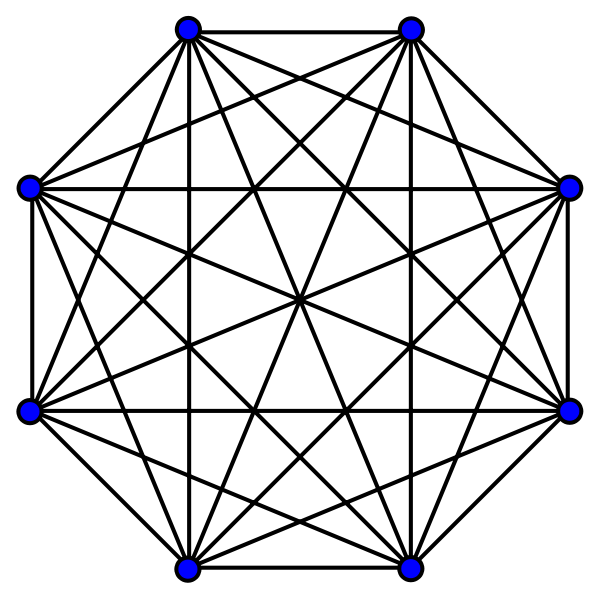
\includegraphics[width=.4\textwidth]{data/complete-graph.png}
		\caption{Exemplo de um grafo completo, isto é, com ligações entre todos os vértices.}
		\label{fig}
	\end{figure}

Como o objetivo é encontrar a melhor rota, cada indivíduo, tem seu material genético representando uma rota. A rota é nada mais que um conjunto de vértices, onde a primeira característica representa o vértice de partida, as proximas características representam os próximos vértices do trajeto, e a ultima característica, representa o vértice de chegada.

Para a implementação do algoritmo, foram usadas as classes \texttt{Element} (que representa um individuo), a classe \texttt{Graph}, representando um grafo, a classe \texttt{Util}, que contem métodos de suporte, como métodos para gerar grafos aleatórios, assim como também métodos para gerar códigos genéticos aleatórios, sendo possível criar indivíduos com dados aleatórios.

Por fim, foi criada também a classe \texttt{GeneticAlgorithm}, que representa o algoritmo genético em si. Essa classe possui métodos para criar uma população de indivíduos aleatórios, métodos para mutar, cruzar e selecionar indivíduos, além de um método chamando estes métodos anteriores em sequência, a fim de executar o algoritmo (método \texttt{run}).


A classe \texttt{GeneticAlgorithm} possui também dados de entrada para o método de instanciação da classe. Esses dados são: \texttt{graph} (o grafo), \texttt{number\_of\_generations} (número de gerações), \texttt{pop\_length} (tamanho máximo da população), \texttt{cross\_rate} (taxa de cruzamento), \texttt{mutation\_rate} (taxa de mutação), \texttt{gen\_range} (taxa de seleção dos indivíduos que irão passar de geração).
Para uma melhor visualização, abaixo está o código desta classe:


\begin{minted}{ruby}
class GeneticAlgorithm
	include Util
	attr_reader :population
	
	#gen_range is a rate of the worst elements that will be eliminated.
	#if it is 20%, 80% of the best elements will paste to the next generation.
	def initialize(graph, number_of_generations=20,pop_length=400, 
			cross_rate=10,mutation_rate=10, gen_range=20)
		@number_of_generations = number_of_generations
		@graph = graph
		@population = []
		@pop_length = pop_length
		@cross_rate = cross_rate
		@gen_range = gen_range
		@mutation_rate = mutation_rate
	end

	def run
		gen_population
		@number_of_generations.times{
			mutate
			cross
			select_next_generation
			gen_population
	}
		@population.first #best element
	end

	def gen_population
		genetic_codes = []
		(@pop_length-population.size).times do 
			genetic_codes << random_genetic_code(@graph.size)
		end
		genetic_codes.uniq!
		genetic_codes.each so |genetic_code| 
			@population << Element.new(genetic_code,@graph) 
		end
		sort_population
	end

	def select_next_generation
		count = calculate @gen_range
		count.times {@population.pop}
	end

	def cross
		(calculate @cross_rate).times do |i| 
			@population.concat(@population[i].crossing(@population[i+1]))
		end
		sort_population
	end

	def mutate
		(calculate @mutation_rate).times do |i|
			j = Random.rand(@population[i].genetic_code.length)
			next if j == 0
			if @population[i].genetic_code.length == @graph.size
				@population[i].genetic_code.delete_at j
			else
				@population[i].genetic_code.insert(j, new_gen(i))
			end
		end
	end

	def new_gen i
		ng = 0
		while @population[i].genetic_code.include? ng
			ng = Random.rand(@population[i].genetic_code.length)
		end
		ng
	end

	def sort_population
		@population.sort!
	end

	def calculate rate
		((@population.size/100)*rate)
	end

end
\end{minted}

É possível visualizar no método run, primeiramente a chamada ao método \texttt{gen\_population}, a fim de criar a população inicial. Após isso, são chamados, dentro de um loop, consecutivamente, os métodos: \texttt{mutate}, \texttt{cross}, \texttt{select\_next\_generation}, \texttt{gen\_population}.

É importante observar que a variável que controla a execução do \emph{loop} é a variável de instância \texttt{number\_of\_generations} (número de gerações). Dentro deste \emph{loop}, o algoritmo irá consecutivamente mutar os indivíduos da população, cruzar, selecionar os que passarão para a próxima geração, gerar novos indivíduos aleatórios e adicioná-los a população.

Agora será explicado o funcionamento da mutação implementada. De começo, obtém-se um índice aleatório, o qual representa o índice de um dos genes do indivíduo. Após isso, há duas condições a considerar: se o tamanho do cromossomo é máximo (passa por todas as cidades) ou não. Caso a primeira proposição for verdadeira, um gene do cromossomo será removido; caso não seja, um novo gene aleatório e não repetitivo será gerado e inserido no código genético do cromossomo em questão, exatamente na posição sorteada primeiramente. Todos esses passos se repetem várias vezes, conforme o valor da variável \texttt{@mutation\_rate} (taxa de mutação).

O cruzamento neste algoritmo é relativamente simples. Primeiramente, é gerado aleatoriamente um índice, para acessar uma característica no vetor que representa o material genético. Em seguida, é trocado a característica representada neste índice nos materias geneticos dos pais, gerando 2 novos materias genéticos, que são usados para criar 2 novos indivíduos e adicioná-los a população. Um ponto a destacar é que as rotas podem ter diferentes quantidades de vértices intermediários (porém nunca mudando o começo e o fim). Isso faz com que sejam gerados indivíduos com material genético de tamanhos diferentes, porém, somente indivíduos com material genético do mesmo tamanho cruzarão. 
Outro ponto a observar é que não é admitido no trajeto passar duas vezes sobre um mesmo ponto, sendo assim, se o cruzamento gerar um individuo em que no seu código genético possui dois vértices iguais, o indivíduo é dito como inválido e não é adicionado a população.
